%%
%% Automatically generated file from DocOnce source
%% (https://github.com/doconce/doconce/)
%% doconce format latex issue160.do.txt 
%%


%-------------------- begin preamble ----------------------

\documentclass[%
oneside,                 % oneside: electronic viewing, twoside: printing
final,                   % draft: marks overfull hboxes, figures with paths
chapterprefix=true,      % "Chapter" word at beginning of each chapter
open=right,              % start new chapters on odd-numbered pages
10pt]{book}

\listfiles               %  print all files needed to compile this document

\usepackage{relsize,epsfig,makeidx,color,setspace,amsmath,amsfonts,amssymb}
\usepackage[table]{xcolor}
\usepackage{bm,ltablex,microtype}

\usepackage{graphicx}
\usepackage{sidecap}

% Movies are handled by the href package
\newenvironment{doconce:movie}{}{}
\newcounter{doconce:movie:counter}


\usepackage[T1]{fontenc}
%\usepackage[latin1]{inputenc}
\usepackage{ucs}
\usepackage[utf8x]{inputenc}

\usepackage{lmodern}         % Latin Modern fonts derived from Computer Modern

% Hyperlinks in PDF:
\definecolor{linkcolor}{rgb}{0,0,0.4}
\usepackage{hyperref}
\hypersetup{
    breaklinks=true,
    colorlinks=true,
    linkcolor=linkcolor,
    urlcolor=linkcolor,
    citecolor=black,
    filecolor=black,
    %filecolor=blue,
    pdfmenubar=true,
    pdftoolbar=true,
    bookmarksdepth=3   % Uncomment (and tweak) for PDF bookmarks with more levels than the TOC
    }
%\hyperbaseurl{}   % hyperlinks are relative to this root

\setcounter{tocdepth}{3}  % levels in table of contents

% Tricks for having figures close to where they are defined:
% 1. define less restrictive rules for where to put figures
\setcounter{topnumber}{2}
\setcounter{bottomnumber}{2}
\setcounter{totalnumber}{4}
\renewcommand{\topfraction}{0.95}
\renewcommand{\bottomfraction}{0.95}
\renewcommand{\textfraction}{0}
\renewcommand{\floatpagefraction}{0.75}
% floatpagefraction must always be less than topfraction!
% 2. ensure all figures are flushed before next section
\usepackage[section]{placeins}
% 3. enable begin{figure}[H] (often leads to ugly pagebreaks)
%\usepackage{float}\restylefloat{figure}

% prevent orhpans and widows
\clubpenalty = 10000
\widowpenalty = 10000

% Redefine double page clear to make it a blank page without headers
% (from BYUTextbook)
\makeatletter
\def\cleardoublepage{\clearpage\if@twoside \ifodd\c@page\else
\hbox{}
\thispagestyle{empty}
\newpage
\if@twocolumn\hbox{}\newpage\fi\fi\fi}
\makeatother
% These commands fiddle with the space left for page numbers in the TOC
% (from BYUTextbook)
\makeatletter
%\renewcommand{\@pnumwidth}{2em}
%\renewcommand{\@tocrmarg}{2.85em}
\makeatother

% Make sure blank even-numbered pages before new chapters are
% totally blank with no header
\newcommand{\clearemptydoublepage}{\clearpage{\pagestyle{empty}\cleardoublepage}}
%\let\cleardoublepage\clearemptydoublepage % caused error in the toc

% --- end of standard preamble for documents ---


% insert custom LaTeX commands...

\raggedbottom
\makeindex
\usepackage[totoc]{idxlayout}   % for index in the toc
\usepackage[nottoc]{tocbibind}  % for references/bibliography in the toc

%-------------------- end preamble ----------------------

\begin{document}

% matching end for #ifdef PREAMBLE

\newcommand{\exercisesection}[1]{\subsection*{#1}}

\renewcommand{\u}{\pmb{u}}
\newcommand{\f}{\bm{f}}
\newcommand{\xbm}{\bm{x}}
\newcommand{\normalvecbm}{\bm{n}}
\newcommand{\ubm}{\bm{u}}

\newcommand{\x}{\pmb{x}}
\newcommand{\normalvec}{\pmb{n}}
\newcommand{\Ddt}[1]{\frac{D#1}{dt}}
\newcommand{\halfi}{1/2}
\newcommand{\half}{\frac{1}{2}}
\newcommand{\report}{test report}

% ------------------- main content ----------------------

\chapter{Commands to be commented out}

\begin{SCfigure}
  \centering
  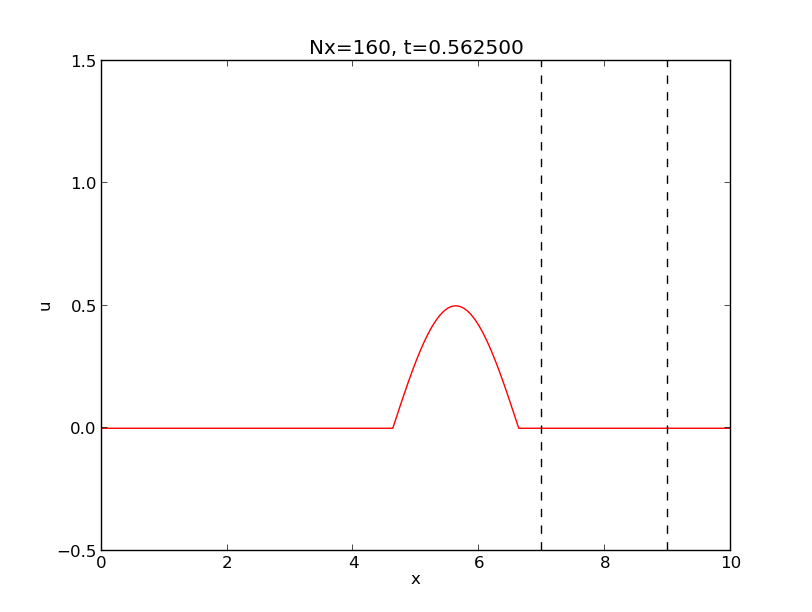
\includegraphics[width=0.9\linewidth]{../doc/src/manual/fig/wave1D.png}
  \caption{
  Figure caption
  }
\end{SCfigure}
%\clearpage % flush figures 


\begin{doconce:movie}
\refstepcounter{doconce:movie:counter}
\begin{center}
\href{{https://www.youtube.com/embed/P8VcZzgdfSc}}{\nolinkurl{https://www.youtube.com/embed/P8VcZzgdfSc}}
\end{center}

\begin{center}  % movie caption
Movie \arabic{doconce:movie:counter}: youtube movie
\end{center}
\end{doconce:movie}



\begin{doconce:movie}
\refstepcounter{doconce:movie:counter}
\begin{quote}
% link to external viewer
Movie \arabic{doconce:movie:counter}: local movie \href{run:../doc/src/manual/mov/wave.webm}{\nolinkurl{../doc/src/manual/mov/wave.webm}}
\end{quote}
\end{doconce:movie}


% ------------------- end of main content ---------------

\end{document}

